\documentclass[]{report}
\usepackage[hmargin=1.25in,vmargin=1in]{geometry} %调整页边距
% \usepackage[inner=1in,outer=1.25in]{geometry} %书籍左右不等宽排版
\usepackage[utf8]{inputenc}
\usepackage[]{ctex} %据说可以直接调用诸如 \kaishu \fangsong \heiti 的命令修改字体
\usepackage[svgnames]{xcolor} % Using colors
% \usepackage{background} % To include background images
\usepackage{fancyhdr} % Needed to define custom headers/footers
\usepackage[]{xeCJK}
\setCJKmainfont[BoldFont = STHeiti, ItalicFont = STKaiti]{Songti SC Light} %中文主字体
\setCJKsansfont[BoldFont = Weibei SC, ItalicFont = HanziPen SC]{Xingkai SC Light} %中文无衬线字体
\setCJKmonofont[BoldFont = Libian SC, ItalicFont = STFangsong]{Yuanti SC Light} %中文等宽字体
\setmainfont{Times New Roman} %\rmfamily
\setsansfont[ItalicFont = American Typewriter]{Comic Sans MS} %\sffamily
\setmonofont{Courier} %\ttfamily
\newfontfamily\monaco{Courier} % 用于代码段字体设置
\newfontfamily\OldCaption{Bodoni 72 Smallcaps Book} %用于全大写字母的标题
\usepackage{titlesec}
% 一下为适用于笔记/整理的板式(第几章-第几节)
\titleformat{\chapter}{\centering\huge\bfseries}{第~\thechapter~章}{1em}{}
\titleformat{\section}{\Large\bfseries}{第~\thesection~节}{1em}{}
% 一下为适用于作业的板式(第几次-第几题-abcd问)
% \titleformat{\chapter}{\centering\huge\bfseries}{第~\thechapter~次作业}{1em}{}
% \titleformat{\section}{\Large\bfseries}{第~\thesection~题}{1em}{}
% \renewcommand{\thesubsection}{(\alph{subsection})}
\usepackage{lipsum} %填充文本

\usepackage{ulem} %解决下划线、删除线之类的
\usepackage{listings}
\lstset{
language=C++,
numberstyle = \monaco,
basicstyle = \monaco,
keywordstyle = \color{blue}\bfseries,
commentstyle=\color[HTML]{006400},
tabsize = 4,
%backgroundcolor=\color{bg}
emph = {int,float,double,char},emphstyle=\color{cyan},
emph = {[2]const, typedef},emphstyle = {[2]\color{red}} }

\makeatletter
\newif\if@restonecol
\makeatother
\let\algorithm\relax
\let\endalgorithm\relax
\usepackage[linesnumbered,ruled,vlined]{algorithm2e}%[ruled,vlined]{
\usepackage{algpseudocode}
\usepackage{amsmath}
\renewcommand{\algorithmicrequire}{\textbf{Input:}}  % Use Input in the format of Algorithm
\renewcommand{\algorithmicensure}{\textbf{Output:}} % Use Output in the format of Algorithm

\usepackage{amsmath} %数学公式问题
\usepackage{amsthm} %公式环境,如proof
\usepackage{booktabs} %三线表
\newcommand{\tabincell}[2]{\begin{tabular}{@{}#1@{}}#2\end{tabular}} %解决单元格内部换行的问题
% 比如这个 Beijing & 0,5 & 1,6 & 2,7 & 3,8 & 4,9 & The number changes every 3 months \\
% 改成这个 \tabincell{l}{Beijing}& \tabincell{c}{0,5}& \tabincell{c}{1,6}& \tabincell{c}{2,7}& \tabincell{c}{3,8}& \tabincell{c}{4,9}& \tabincell{c}{The number changes \\ every 3 months} \\
% 一个单元格过长,整行都需要修改
% 可以配合 \resizebox*{h-width}{v-width}{contents, e.g.tabular} 使用

\usepackage{mathrsfs} %在公式里面使用那个最花的字体
\usepackage{amssymb} %公式里面用空心黑体和旧式字体
\usepackage{amssymb} %AMS符号
\usepackage{amsthm} %AMS定理环境

\usepackage{markdown} %使用markdown语法,在编译时需要打开 shell-escape 标记,即 $ xelatex --shell-escape example.tex
\markdownSetup{hashEnumerators = true} %允许使用 #. 的方式编写有序列表
\markdownSetup{inlineFootnotes = true} %允许使用脚注形式的超链接,调用语法为 [anchor](uri), ^[footnote], <uri>
\markdownSetup{fencedCode = true} %以反引号和缩进来插入代码段,相当于 verbatim
\markdownSetup{
  pipeTables = true
} %支持表格的用法 (图片已经在markdown包里面支持了)
% \usepackage{booktabs} %解决三线表的线条粗细问题

\usepackage{graphicx} %插入图片
\usepackage{pdfpages} %插入PDF文件
\usepackage{makeidx}

\usepackage{tikz} %带圈字符
\usepackage{etoolbox} %带圈字符 (提供robustify)
\usepackage{enumitem}
\newcommand*{\circled}[1]{\lower.7ex\hbox{\tikz\draw (0pt, 0pt)%
    circle (.5em) node {\makebox[1em][c]{\small #1}};}} %新定义命令:带圈字符
\robustify{\circled}
% \usepackage{enumerate} %有序列表

\usepackage{hyperref} %超链接
% \usepackage[hidelinks]{hyperref} %隐藏超链接的红框
\markdownSetup{
  inlineFootnotes = true,
  renderers = {
    link = {\href{#3}{#1}},
  }
} % markdown块中使用直接点进去的超链接
% \setlist[enumerate,1]{label=(\arabic*).,font=\textup,leftmargin=7mm,labelsep=1.5mm,topsep=0mm,itemsep=-0.8mm}
% \setlist[enumerate,2]{label=(\alph*).,font=\textup,leftmargin=7mm,labelsep=1.5mm,topsep=-0.8mm,itemsep=-0.8mm}

\usepackage{braket}

%%%%%% Setting up the style

% \setlength\parindent{0pt} % Gets rid of all indentation
% \backgroundsetup{contents={\includegraphics[width=\textwidth]{ustc-name.pdf}},scale=0.4,placement=top,opacity=0.6,color=cyan,vshift=-20pt} %  USTC Logo

\pagestyle{fancy} % Enables the custom headers/footers

% 使用默认的Chapter页眉
% \lhead{} \rhead{} % Headers - all  empty

% \title{\vspace{-1.8cm}  \color{DarkRed} Laboratory Rotation Report}
% \subtitle{Title of the proposal % Title of the rotation project
% \vspace{-2cm} }
% \date{\today} % No date

\lfoot{\color{Grey} \textit{上官凝}}  % Write your name here
\rfoot{ \color{Grey} 随机过程笔记 }
\cfoot{\color{Grey} \thepage}

\renewcommand{\headrulewidth}{0.0pt} % No header rule
\renewcommand{\footrulewidth}{0.4pt} % Thin footer rule

\title{随机过程笔记}
\author{上官凝}
\date{\today}

\linespread{1.3} %行间距为1.3倍默认间距 (1.3 x 1.2倍字符宽度)

\makeindex

\begin{document}
\theoremstyle{definition} \newtheorem{theorem}{Thm}[section] %定义一个定理Thm,序号为section的下一级序号
\theoremstyle{definition} \newtheorem{definition}{Def}[section] %定义一个定义Def,序号为section的下一级序号
\theoremstyle{plain} \newtheorem{lemma}{lemma}[section] %引理

	\maketitle
	\newpage

	\tableofcontents
	\newpage

	\chapter{引论}
	\section{引言}
		\begin{definition}[严格平稳\label{严平稳}]
			如果随机过程$X(t)$对任意的$t_1,\cdots,t_n\in T$和任何$h$有
			\[(X(t_1+h),\cdots,X(t_n+h))\stackrel{d}{=}(X(t_1),\cdots,X(t_n)),\]则称为严格平稳的
		\end{definition}
		\begin{definition}[宽平稳\label{宽平稳}]
			如果随机过程的所有二阶矩存在并有$EX(t)=m$及协方差函数$R_X(t,s)$只与时间差$t-s$有关,则称为宽平稳的或二阶平稳的
		\end{definition}
		\begin{definition}[\textbf{独立增量过程}\label{独立增量过程}]
			如果对任意的$t_1<t_2\cdots<t_n,t_1,\cdots,t_n\in T$,随机变量$X(t_2)-X(t_1),X(t_3)-X(t_2),\cdots,X(t_n)-X(t_{n-1})$是相互独立的,则称$X(t)$为\textbf{独立增量过程}。如果进一步有对任意的$t_1,t_2,X(t_1+h)-X(t_1)\stackrel{d}{=}X(t_2+h)-X(t_2)$,则过程称为有平稳独立增量的过程
		\end{definition}
	\section{条件期望与矩母函数}
		对于连续型随机变量,定义其条件概率为:
		\[P(X\in A\mid Y=y)=\lim_{\Delta y\downarrow0}P(X\in A\mid Y\in\Delta y)\]\par
		条件期望的表达式为:
		\[E(X\mid Y=y)=\sum_xxP\{X=x\mid Y=y\}\qquad(\mbox{离散型随机变量Y})\]
		\[E(X\mid Y=y)=\int xf(x\mid y)\,dx\qquad\mbox{连续型随机变量Y}\]
		\[E(X\mid Y=y)=\int x\,dF(x\mid y)\qquad\mbox{统一记作这个}\]\par
		条件期望的性质有:
		\begin{enumerate}
			\item 若$X$和$Y$独立,则$E(X\mid Y=y)=EX$
			\item 条件期望有所谓的平滑性:\[EX=\int E(X\mid Y=y)\,dF_Y(y)=E[E(X\mid Y)]\]
			\item 对随机变量$X,Y$的函数$\phi(X,Y)$恒有\[E(\phi(X,Y)\mid Y=y)=E(\phi(X,y)\mid Y=y)\]
		\end{enumerate}\par
		\begin{definition}[矩母函数]
			随机变量$X$的矩母函数定义为随机变量$\exp{tX}$的期望,记作$g(t)$,即
			\[g(t)=E(\exp\{tx\})=\int\exp\{tx\}\,dF(x)\]
		\end{definition}
		通过矩母函数可以求出$X$的各阶矩,即有
		\[E[X^n]=g^{(n)}(0),\quad n\ge1\]
		而对相互独立的随机变量$X$和$Y$,他们和的矩母函数就等于其矩母函数的积:
		\[g_{X+Y}(t)=g_{X}(t)g_{Y}(t)\]
		\begin{definition}[生成函数]
			若$X$为离散随机变量,则期望$E(s^X)$为其概率生成函数,记作$\phi_X(s)$。特别地,若$P(X=k)=p_k,k=0,1,2,\cdots$,则$\displaystyle\phi_X(s)=\sum_{k=0}^{\infty}p_ks^k$
		\end{definition}
		\paragraph{随机和的矩母函数(例 1.12)} 记$X_1,X_2,\cdots$为一串独立同分布的随机变量,$N$为非负整数值随机变量且与$X$序列相互独立。$Y$为随机和$\displaystyle\sum_{i=1}^NX_i$。求$Y$的矩母函数$g_Y(t)$
		\begin{figure}[h!]
			\centering
			\begin{minipage}{40em}
				\centering
				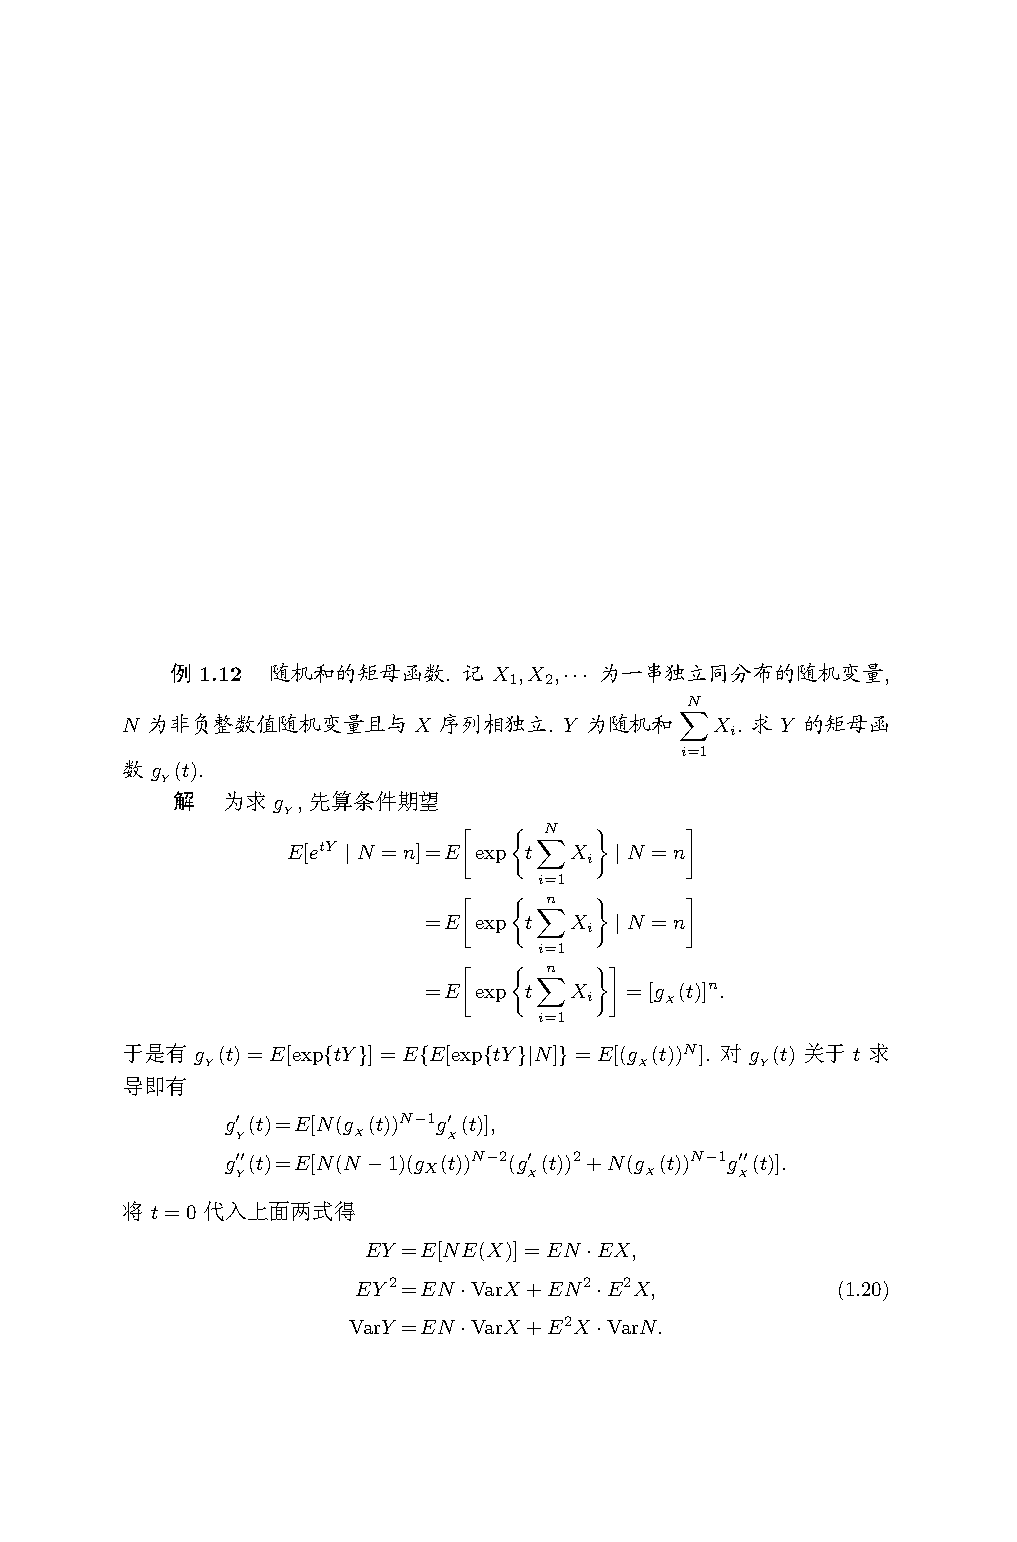
\includegraphics[scale = 0.9]{images/随机和的矩母函数.pdf}
			\end{minipage}
		\end{figure}

	\chapter{Poisson过程}
	本章的符号:
	\begin{enumerate}
		\item $X_n$:第$n-1$次与第$n$次事件间的间隔时间
		\item $W_n=\displaystyle\sum_{i=1}^nX_i$为第$n$次事件的到达或等待时间
	\end{enumerate}\par
	一定要记住,Poisson的Poisson是对于\textbf{区间上的事件发生}而言的。
	\section{Poisson过程}
		Poisson过程有如下两个性质:一是在时间或空间上的均匀性,二是未来的变化与过去的变化没有联系
		\begin{definition}[Poisson过程]
			一个整数值随机变量$\{N(t),t\ge0\}$满足下述三个条件就称作强度为$\lambda>0$的Poisson过程:
			\begin{enumerate}
				\item $N(0)=0$
				\item $N(t)$是独立增量过程(其定义如\ref{独立增量过程}所示)
				\item 对任何$t>0,s\ge0$,增量$N(s+t)-N(s)$服从参数为$\lambda t$对Poisson分布,即\[P\{N(s+t)-N(s)=k\}=\frac{(\lambda t)^k\exp\{-\lambda t\}}{k!},k=0,1,\cdots\]
			\end{enumerate}
		\end{definition}\par
		\begin{definition}[Poisson过程的假定\label{Poisson过程的假定}]
			对于Poisson过程,我们有如下四条\textbf{充分必要的}假定\textit{(注意和后面其变种的区别)}:
			\begin{enumerate}
				\item 在不相交区间中事件发生的数目相互独立,也即对任何整数$n=1,2,\cdots$,设时刻$t_0=0<t_1<t_2<\cdots<t_n$,增量$N(t_1)-N(t_0),N(t_2)-N(t_1),\cdots,N(t_n)-N(t_{n-1})$相互独立。\textit{为前后的独立性,说明试验是独立的}
				\item 对任何时刻$t$和正数$h$,随机变量(增量)$N(t+h)-N(t)$对分布只依赖于区间长度$h$而不依赖于时刻$t$。\textit{为时间上的均匀性或齐次性,说明在每个长度相同的小区间上事件有着相同的概率$p$}
				\item 存在正常数$\lambda$,当$h\downarrow0$时,在长度为$h$的小区间中事件至少发生一次的概率为\[P\{N(t+h)-N(t)\ge1\}=\lambda h+o(h)\]\textit{事件是稀有的,其发生概率为$p=\lambda h$,而且$p$很小}
				\item 在长度为$h$的小区间上发生两个或两个以上事件的概率为$o(h)$,即\[\lim_{h\downarrow0}P\{N(t+h)-N(t)\ge2\}=o(h)\]\textit{为相继性,指事件是一件一件地发生的,在同一时间同时发生多个事件的可能性很小很小,而不发生的概率为$1-\lambda h=1-p$}
			\end{enumerate}
		\end{definition}
	\section{与Poisson过程相联系的若干分布}
		下面这个样本累计图对理解和掌握Poisson过程十分有用:
		\begin{figure}[ht!]
			\centering
			\begin{minipage}{40em}
				\centering
				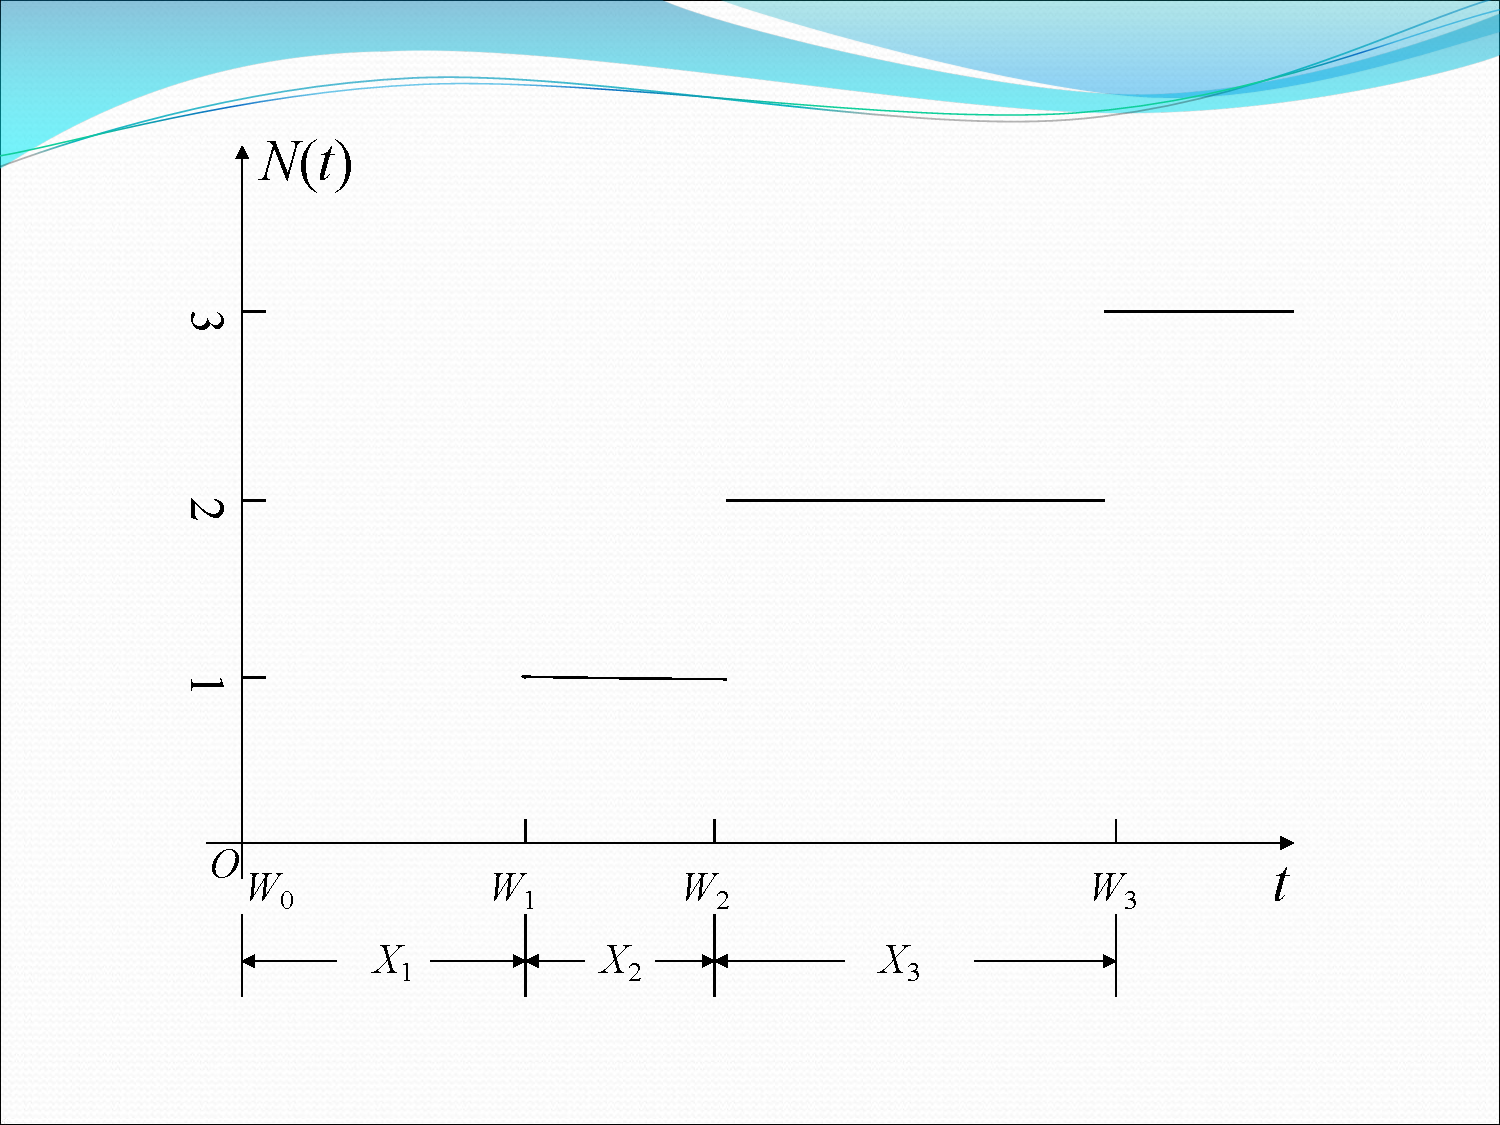
\includegraphics[scale = 0.5]{images/Poisson过程的样本路径.pdf}
				\caption{Poisson过程的样本路径}
			\end{minipage}
		\end{figure}
		\begin{theorem}[一条很重要的性质]
		\[\boxed{P\{W_n\le t\}=P\{N(t)\ge n\}=\sum_{j=n}^\infty e^{-\lambda t}\frac{(\lambda t)^j}{j!}}\]
		即事件$\{N(t)\ge n\}$是与$W_n\le t$等价的,它们都表明第$n$次事件发生在时刻$t$之前,或者换言之,到时刻$t$已经发生了$n$件事
		\end{theorem}
		\[X_1,X_2,\cdots,X_n\ i.i.d\sim exp(\frac{1}{\lambda})\]
		\[W_n\sim\varGamma(n,\lambda)\]
		\[f_{W_n}(t)=\lambda e^{-\lambda t}\frac{(\lambda t)^{n-1}}{(n-1)!}\]
		\begin{theorem}
			若$N(t),t\ge0$为Poisson过程,则给定$N(t)=n$下等待时间$W_1,\cdots,W_n$的联合密度为
			\[f_{W_1,\cdots,W_n\mid N(t)=n}(\omega_1,\cdots,\omega_n\mid n)=\frac{n!}{t^n},\ 0<W_1<\cdots<W_n\le t\]
		\end{theorem}
	\section{Poisson过程的推广}
		\subsection{非齐次Poisson过程}
			当允许强度$\lambda$(即事件在某一小区间上的概率与区间长度的比例因子)依赖于时刻$t$,这提供了过程增量不平稳的例子,此时,
			\[P\{N(t+h)-N(t)=k\}=\frac{(\int_{t}^{t+h}\lambda(u)\,du)^k\exp(\int_{t}^{t+h}\lambda(u)\,du)}{k!},k=0,1,\cdots\]\par
			非齐次Poisson过程的假定只需要将\ref{Poisson过程的假定}中第二条去掉,并将(3)换为
			\[P\{N(t+h)-N(t)\ge1\}=\lambda(t)h+o(h)\]
		\subsection{复合Poisson过程}
			累计值过程$X(t)=\displaystyle\sum_{i=1}^{N(t)}Y_i$,其中$Y_i$为独立同分布的随机变量,有分布函数$G(y)$,期望$EY=\mu$,方差$VarY=\tau^2$。$N(t)$是参数为$\lambda$的Poisson过程。则$X(t)$就是复合Poisson过程,他是随机和并且$E[X(t)]=\lambda\mu t,Var[X(t)]=\lambda(\tau^2+\mu^2)t$
		\subsection{更新过程}
			将时间间隔$X_i$服从的指数分布改为一般的分布函数$F(x)$,就得到所谓的更新过程

	\chapter{Markov过程}
	独立随机实验模型最直接的推广就是Markov链模型。粗略而言,一个随机过程如果给定了当前时刻$t$的值$X_t$,未来$X_s(s>t)$的值不受过去的值$X_u(u<t)$的影响就称为有Markov性。\par
	记号:
	\begin{enumerate}
		\item 当$X_n=i$,就称过程在时间$n$处于状态$i$
		\item 转移概率矩阵$P=(P_{ij})$,矩阵的第$i+1$行就是给定$X_n=i$时,$X_{n+1}$的概率分布
		\item 一步转移概率$P_{ij}^{n,n+1}$和一步转移概率矩阵$P^{n,n+1}$(当此矩阵与$n$无关时成为上面的$P$)
		\item n步转移概率和n步转移概率矩阵$P^{(n)}$
	\end{enumerate}
	\section{Markov链的定义和例子}
		\begin{definition}[Markov性质]
			如果对任何一列状态$i_0,i_1,\cdots,i_{n-1},i_n,j$,以及对任何$N\ge0$,随机过程$\{X_n,n\ge0\}$满足Markov性质
			\[P\{X_{n+1}=j\mid X_0=i_0,X_1=i_1,\cdots,X_{n-1}=i_{n-1},X_n=i\}=P\{X_{n+1}=j\mid X_n=i\}\]
			则称$X_n$为\textit{离散时间}Markov链
		\end{definition}
		\begin{definition}[平稳转移概率]
			平稳转移概率$P_{ij}^{n,n+1}$为从($X_n$,状态i)到($X_{n+1}$,状态j)的转移概率,当此概率与n无关时记为$P_{ij}$,并称为平稳转移概率
		\end{definition}
		\begin{definition}[n步转移概率矩阵]
			n步转移概率矩阵$\mathbf{P}^{(n)}$
			\[\mathbf{P}^{(n)}=\mathbf{P}^n=\sum_{k=0}^\infty P_{ik}P_{kj}^{(n-1)}\]
			\[\mathbf{P}^{(n+m)}=\sum_{k=0}^\infty P_{ik}^{(n)}P_{kj}^{(m)}\]
		\end{definition}
		\begin{theorem}[求n步转移概率矩阵]
			n步转移概率矩阵$P^{(n)}=P^n$
			\[P\{X_0=i_0,X_1=i_1,\cdots,X_n=i_n\}=p_iP_{i_0,i_1}\cdots P_{i_{n-1},i_n}\]\par
			这个结论在直接计算的时候很平凡,但是在证明的时候不一定会想起来
		\end{theorem}
		\subsection{求矩阵的n次方}
		由线性代数的知识可以知道,实对称矩阵一定可以对角化\footnote{《线性代数与解析几何 第二版》陈发来等著,P176 \S{6.4}}。下面对一个n阶的实对称矩阵A进行对角化,即求正交矩阵$T$,使得$T^{-1}AT$为对角矩阵:\footnote{《线性代数与解析几何 第二版》陈发来等著,P208 \S{7.3} 例7.3.1}
		\begin{enumerate}
			\item 求出矩阵A的特征多项式$\det(\lambda I-A)=f_n(\lambda)$为一个关于$\lambda$的n次多项式
			\item 对于n个特征值$\lambda_i$,分别求解$(\lambda_iI-A)x_1=0$
			\item 将$x_i$分别单位化,得到$e_i$(均为列向量)
			\item 将$e_i$自左向右合为一个矩阵,即为$T$
		\end{enumerate}
	\section{Markov链的状态分类}
		\begin{definition}[可达与互达]
			如果对某一$n\ge0$,有$P_{ij}^(n)>0$,则称状态$j$是从状态$i$可达的,记作$i\to j$。他表示从状态$i$经过有限步的转移可以到达状态$j$。两个互相可达的状态$i$和$j$称为互达的,记作$i\leftrightarrow j$
		\end{definition}
		互达性是等价关系。\par
		如果在互达性这一等价关系下Markov链的所有状态都居于同一类,那么称这个Markov链是不可约的
		\begin{definition}[Markov链的周期]
			设i为Markov链的一个状态,使$P_{ii}^{(n)}>0$的所有正整数$n(n\ge1)$的最大公约数称作是状态i的周期,记作$d(i)$。如果对所有$n\ge1$,都有$P_{ii}^{(n)}=0$则约定周期为$\infty$;周期为1的状态非周期的
		\end{definition}
		如果$i\leftrightarrow j$,那么$d(i)=d(j)$
		\begin{theorem}
			如果状态i有周期$d(i)$,那么存在整数N,使得对所有$n>N$恒有$P_{ii}^{(nd(i))}>0$\par
			$P_{ji}^{(m+nd(i))}\ge P_{ji}^{(m)}P_{ii}^{(nd(i))}$\par
			如果$P_{ji}^{(m)}>0$,则存在正整数N,使得对所有$n>N$恒有$P_{ji}^{(m+nd(i))}>0$
		\end{theorem}
		\begin{theorem}
			令P为不可约、非周期、有限状态Markov链的转移矩阵,则必存在N,使得当$n\ge N$时,n步转移概率阵$P^{(n)}$的所有元素都非零
		\end{theorem}
		\begin{definition}[常反和瞬过]
			$f_{ij}^{(n)}$:从i出发在n步转移时首次到达j的概率\par
			$f_{ij}$:从i出发最终转入状态j的概率\par
			如果$j_{ii}=1$(也等价于$\displaystyle\sum_{n=1}^\infty P_{ii}^{(n)}=\infty$),称状态i是常反的
		\end{definition}
		\begin{definition}[常反时、正常反和零常反]
			对常反状态i,定义$T_i$为首次返回状态i的时刻,称作常反时。记$\mu_i=ET_i$,则有
			\[\mu_i=\sum_{n=1}^\infty nf_{ii}^{(n)}\]
			一个常反状态i当且仅当$\mu_i=\infty$时称为零常反的,当且仅当$\mu_i<\infty$时称为正常反的
		\end{definition}
		\subsection{可达、周期、常反的判断}
			可达性、等价类个数可以由Markov链状态转换图直接看出来。周期利用同一个等价类中所有状态周期一样的性质,找一个最好算的。常反可以用$\sum f_{ii}^{(n)}$,找规律来计算,然后利用同一等价类中是否瞬过相同。正常反、零常反、瞬过也可以用下一节第一个定理来判断
	\section{Markov链的极限定理和平稳分布}
	\section{分支过程}
	\section{连续时间Markov链}
		\begin{definition}
			若对所有$s,t\ge0$和任何非负整数$i,j,x(u),0\le u\le s$,随机过程$X(t),t\ge0$,满足
			\[P\{X(t+s)=j\mid X(s)=i,X(x)=x(u),0\le u<s\}=P\{X(t+s)=j\mid X(s)=i\}\]
		\end{definition}\par
		连续时间Markov链的转移概率$P_{ij}(i)$和$p_i$


	\chapter{平稳过程}
	平稳过程$X=\{X(t),t\in T\}$是其概率性质在时间平移下不变的随机过程
	\section{定义和例子}
		回顾一下第一章对于严平稳(\ref{严平稳})和宽平稳(\ref{宽平稳})的定义。\par
		设T是具有以下性质的下标集合(对加法封闭):若$t_1,t_2\in T$,则$t_1+t_2\in T$。通常取以下几种集合之一:
		\begin{enumerate}[label = (\roman{*})]
			\item $T=\{0,1,2,\cdots\};$
			\item $T=\{0,\pm1,\pm2,\cdots\};$
			\item $T=\{t:t\ge0\};$
			\item $T=\{t:-\infty<t<\infty\}.$
		\end{enumerate}
		\begin{definition}[严平稳过程]
			设$X=\{X(t),t\in T\}$为一随机过程,若对任意正整数k及T中任意k个时刻$t_1<\cdots<t_k\in T$和任何$h\in T$有
			\[(X(t_1+h),\cdots,X(t_k+h))\stackrel{d}{=}(X(t_1),\cdots,X(t_k)),\]则随机过程X称为严格平稳过程。
		\end{definition}\par
		如果$T=\{0,\pm1,\pm2,\cdots\}$,我们一般把X称为随机序列。如果X还是严平稳的,则称为严平稳序列。
		\begin{theorem}
			设$X=\{X(t),t\in T\}$为严平稳过程,则:
			\begin{enumerate}[label = (\alph{*})]
				\item $m(t)=EX(t)=m$(期望,是常数若存在)
				\item $Var(X(t))=E(X(t)-m)^2=\sigma^2$(方差,是常数若存在)
				\item $E(X(t)-m)(X(s)-m)=E(X(t-s)-m)(X(0)-m)\stackrel{h=t-s}{=}R(h)$(协方差函数,仅与时间差有关)
				\item $Var(X(t))=R(0)$
				\item $r(\tau)=EX(t)X(t+\tau)$(自相关函数,与起点t无关)
				\item $\rho(v)=R(v)/\sigma^2=R(v)/R(0)$(标准自相关函数,$\rho(0)=1,\mid\rho(v)\mid\le1$)
			\end{enumerate}
			严平稳过程要求所有有限维分布都与起点无关
		\end{theorem}
		\begin{definition}[宽平稳过程]
			设$X=\{X(t),t\in T\}$为一实值随机过程,如果对$\forall t\in T,EX^2(t)<\infty,EX(t)=m$以及协方差函数$E(X(t)-m)(X(s)-m)$仅与$t-s$有关,则称$X$为宽平稳随机过程
		\end{definition}
		\begin{definition}[Gauss过程]
			设$G=\{G(t),-\infty<t<\infty\}$为一随机过程,如果对任一正整数k以及k个时刻$t_i\le t_2\le\cdots\le t_k$,有$(G(t_1),G(t_2),\cdots,G(t_k))$的联合分布为k维正态分布,则称G为Gauss过程
		\end{definition}

\end{document}
